In this section, we will provide an overview of the background knowledge required to understand the rest of this work.
This includes an introduction to the concepts of Adversarial Machine Learning and adversarial examples, as well as an
introduction to the concepts of Intrusion Detection Systems and the challenges they face.

\subsection{Intrusion Detection Systems}\label{subsec:intrusion-detection-systems}
Intrusion Detection Systems (IDS) are security tools designed to identify and prevent unauthorized access, misuse, and
malicious activities in computer networks~\cite{mukherjee1994network}.
IDS play a critical role in protecting networks from various types of cyber threats, including viruses, malware, and
intrusions.
IDS operate by monitoring network traffic and analyzing it for suspicious behavior or patterns.
There are two main types of IDS: Network-based Intrusion Detection Systems (NIDS) and Host-based Intrusion Detection
Systems (HIDS)~\cite{pharate2015classification}.

NIDS monitors network traffic and analyzes packets to identify potential security threats.
NIDS can be deployed at different points within the network, such as at the perimeter, within the LAN, or at critical
points within the network.
NIDS can detect a wide range of attacks, including port scans, denial-of-service attacks, and data exfiltration.

HIDS, on the other hand, monitors the activity on individual hosts, such as servers or workstations.
HIDS can detect attacks that may not be visible to NIDS, such as attacks that occur within encrypted traffic or attacks
that originate from within the network.

From this point on, and to facilitate the understanding of the document, we will refer to Network Intrusion Detection
Systems as Intrusion Detection Systems.

Intrusion Detection Systems are an essential component of a comprehensive network security strategy.
They provide an additional layer of protection beyond firewalls, antivirus software, and other security tools.
By detecting and alerting administrators to potential security threats, IDS can help organizations respond quickly and
effectively to cyber attacks.

Machine Learning (ML) has emerged as a powerful technique for improving the accuracy and effectiveness of Intrusion
Detection Systems~\cite{abdallah2022intrusion, maseer2021benchmarking, thakkar2020review}.
ML algorithms can be used to analyze large volumes of network data and identify patterns that may be indicative of
security threats.
ML-based IDS can learn from past network activity to identify and flag potential security threats in real-time, even
when the attacks are novel or previously unseen.
ML-based IDS can also adapt and improve over time as they learn from new data and feedback from security analysts.

\subsection{Adversarial Machine Learning}\label{subsec:adversarial-machine-learning}

Adversarial Machine Learning (AML) attacks refer to a set of techniques used to undermine the accuracy, integrity, or
security of machine learning (ML) models~\cite{huang2011adversarial}.
AML attacks can be launched by malicious actors with different objectives, such as stealing sensitive information,
manipulating decision-making processes, or compromising the confidentiality and privacy of ML systems.

\begin{figure}
\centering
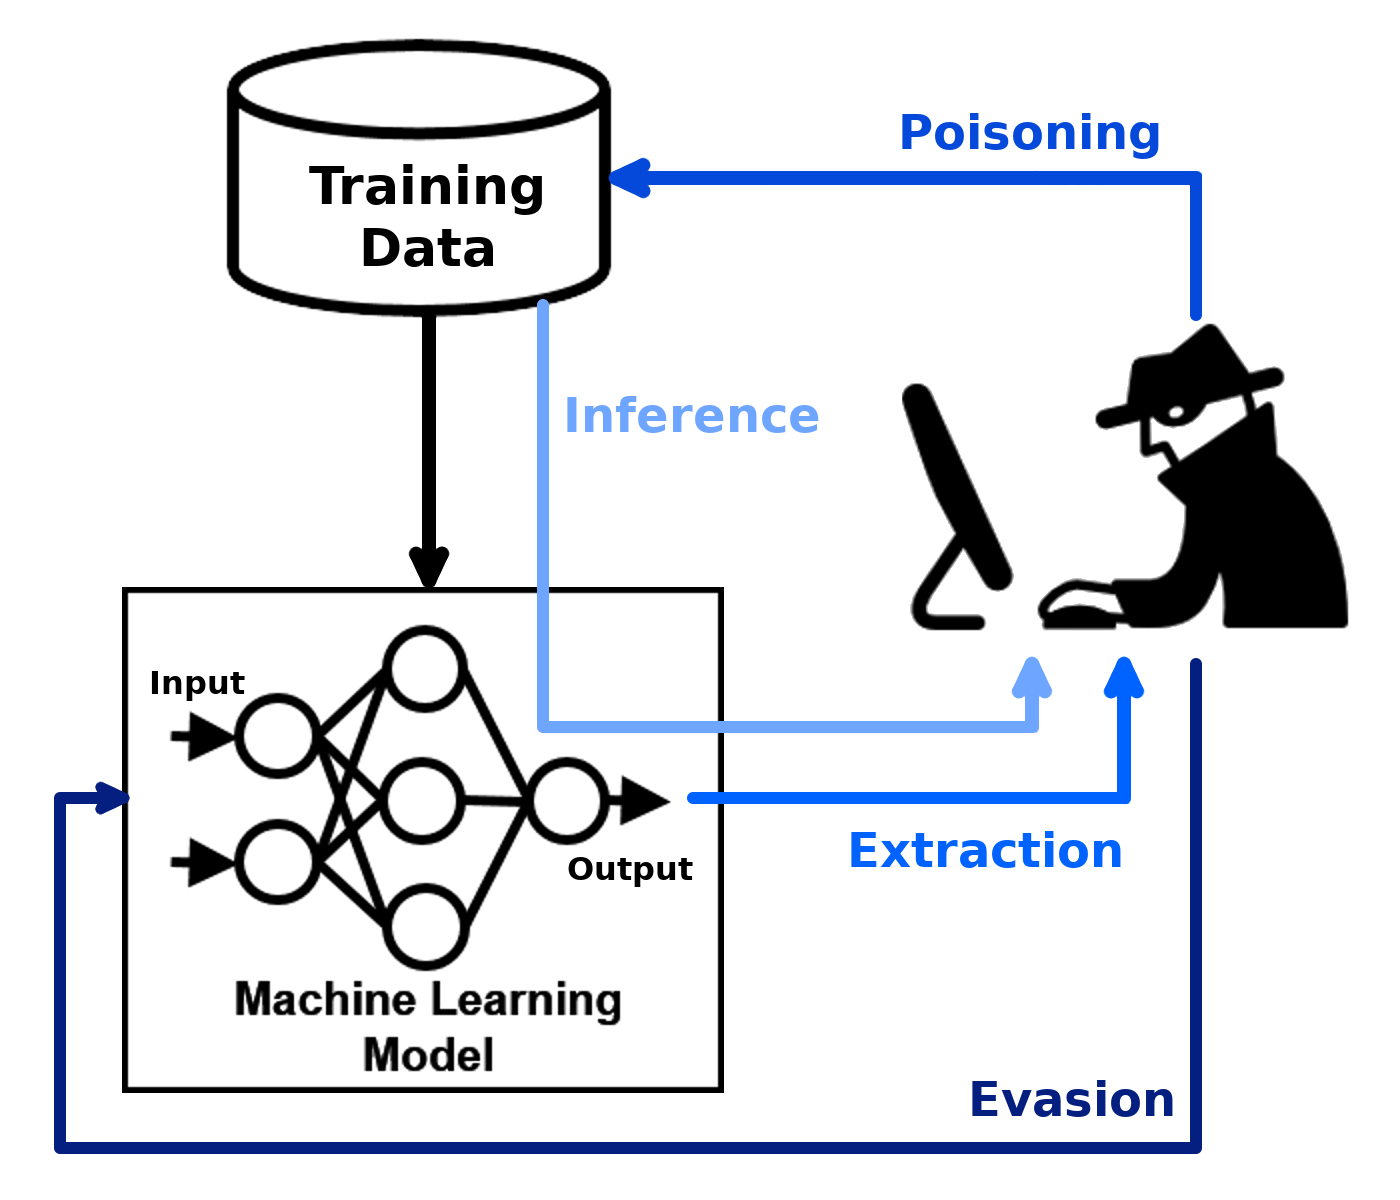
\includegraphics[width=0.9\columnwidth]{AML}
\caption{Adversarial Machine Learning (AML) attacks by ART~\cite{art2018}}
\label{fig:aml}
\end{figure}

AML attacks can be launched against a wide range of ML models, including deep neural networks, support vector machines,
decision trees, and others.
The success of an AML attack depends on various factors, such as the type and quality of the target ML model, the
sophistication of the attack technique, and the attacker's level of knowledge and resources.
According to the taxonomy of the attack, they can be classified into evasion attacks, poisoning attacks, extraction
attacks and inference attacks\cite{de2020overview}.

\subsubsection{Evasion Attacks}
Evasion attacks in AML refer to a type of attack where the attacker manipulates the input data in a way that the ML
model will misclassify it, without changing the underlying characteristics of the data.
Evasion attacks are typically launched against classification models, such as those used for image recognition or spam
detection, and they can be crafted using various techniques, including gradient-based methods, evolutionary algorithms,
or grey/black-box attacks.
The goal of an evasion attack is to create an adversarial example, i.e., a modified version of the original input data
that is similar to the original but is misclassified by the ML model.
Evasion attacks pose a significant threat to the security and robustness of ML systems, especially in domains such as
malware detection, Intrusion Detection Systems and fraud detection, where accurate classification is critical.

\subsubsection{Poisoning Attacks}
Data poisoning attacks in AML involve manipulating the training data of an ML model to introduce biases or to cause it
to learn incorrect patterns.
Poisoning attacks can be launched at different stages of the ML pipeline, including data collection, preprocessing, and
training.
The goal of a poisoning attack is to compromise the integrity and accuracy of the ML model by introducing malicious
data into the training dataset, which can cause the model to learn incorrect patterns and make incorrect predictions.
Poisoning attacks can be launched in a variety of ways, such as by injecting adversarial examples into the training
data, manipulating the distribution of the training data, or introducing outliers into the dataset.

\subsubsection{Extraction Attacks}
Model extraction attacks in AML refer to a type of attack where the attacker aims to extract the details of an ML model
without direct access to it.
This is achieved by leveraging the output of the target ML model to infer the underlying structure, architecture, or
parameters of the model.
Model extraction attacks can be launched through different channels, such as querying the model with carefully crafted
inputs or by observing its behavior in response to various inputs.
The goal of a model extraction attack is to steal the target model's intellectual property or use it for malicious
purposes such as deploying counterfeit models, stealing sensitive data, or reverse engineering proprietary algorithms.
Model extraction attacks can be particularly effective against black-box models where the attacker does not have access
to the model's internal structure or parameters.

\subsubsection{Inference Attacks}
AML inference attacks involve an attacker attempting to glean confidential information about the input data utilized
by the ML model by scrutinizing the model's output.
Inference attacks can be launched against a wide range of ML models, including deep neural networks, decision trees,
and support vector machines, among others.
The goal of an inference attack is to obtain access to private or confidential information about the input data, such
as personal characteristics, financial transactions, or medical records, without having direct access to the data itself.
Inference attacks can be launched through different channels, such as analyzing the output distribution of the model,
measuring its response time to different inputs, or exploiting the model's decision boundaries.


\subsection{Multi-Armed Bandits (MAB)}\label{subsec:back-multi-armed-bandit}
The \textit{Multi-Armed Bandits (MAB)} is a classic problem in probability theory and Machine Learning, where an agent
has to allocate a limited set of resources among competing choices that have uncertain
rewards~\cite{kuleshov2014algorithms}.
The agent faces a trade-off between exploiting the choices that have the highest expected rewards based on the current
information, and exploring new choices that may yield higher rewards in the future.

The \textit{MAB} problem has many practical applications in various domains, such as clinical trials, adaptive routing,
financial portfolio design, and online advertising.
Several algorithms have been proposed to solve the \textit{MAB} problem, such as optimistic
initialization~\cite{machado2014domain}, upper confidence bound (UCB)~\cite{carpentier2011upper}, and
Thompson sampling~\cite{agrawal2012analysis}.
These algorithms differ in how they balance exploration and exploitation, and how they estimate the expected rewards of
each choice.

Thompson sampling is a Bayesian approach that maintains a probability distribution over the unknown reward distributions
of each choice, and chooses actions based on sampling from these distributions.
Specifically, at each timestep, Thompson sampling samples a reward from each distribution, chooses the action associated
with the highest sampled reward, and updates its beliefs about the reward distributions based on the observed reward.
This approach has been shown to be effective in many applications, and has a strong theoretical justification in terms
of minimizing regret.

Thompson sampling has gained popularity in recent years due to its ability to balance exploration and exploitation in a
principled way~\cite{park2021analysis}.
By sampling from the probability distributions over the reward distributions, Thompson sampling encourages exploration
of all choices while still favoring choices with higher expected rewards.
Additionally, the Bayesian framework allows for the incorporation of prior knowledge about the reward distributions,
which can be especially useful in scenarios with limited data.

The \textit{MAB} problem is intricately connected to the realm of Reinforcement Learning (RL).
In RL, an intelligent agent endeavors to acquire knowledge and develop a strategy, known as a policy, that maximizes
its total rewards throughout its interaction with an environment.
Over the past few years, RL has exhibited remarkable success in diverse domains.
Notably, it has found significant utility in the domain of demand forecasting~\cite{ramos2022selection, ramos2022learning}.

In the context of our work, we use the \textit{MAB} algorithm to select the best (IDS) classifier for each network traffic
request. 
This is similar to how \textit{MAB} is used in demand forecasting to select the most optimal forecasting model or determine
the best hyperparameters for a given forecasting model.
By using \textit{MAB}, we can balance the trade-off between exploiting the classifiers that have the highest expected
accuracy based on the current information, and exploring new classifiers that may yield higher accuracy in the future.